\documentclass{article}
\usepackage[utf8]{inputenc}
\usepackage{graphicx}

\title{Tarea 2}
\author{Sergio Adair López Sánchez}
\date{Noviembre de 2022}

\begin{document}

\maketitle

\textbf{Problema 5:} La llamada (bundle ’(”a” ”b” ”c”) 0) es un buen uso de bundle? ¿qué produce? ¿por qué?
\\\\
No. Produce un loop infinito, por lo que mejor devolvemos el error:
\begin{verbatim}
   (error 'bundle "n no puede ser menor que 1")
\end{verbatim}

\ \\
\textbf{Problema 9:} Dibuja un diagrama como el de la figura anterior pero para la lista ’(11 9 2 18 12 14 4 1)
\begin{center}
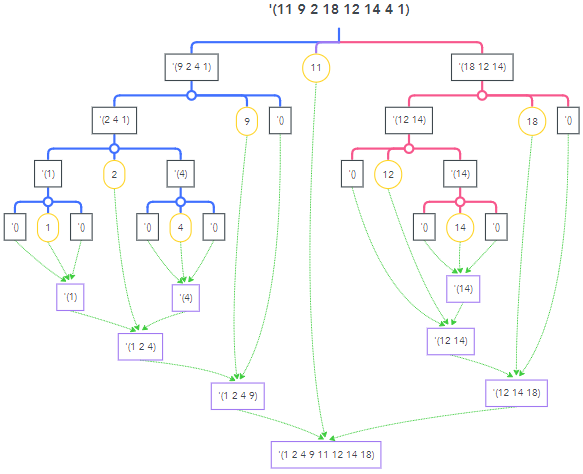
\includegraphics[width=12cm]{diagrama-quicksort.png}
\end{center}
\newpage
\textbf{Problema 11:} Si la entrada a quicksort contiene varias repeticiones de un número, va a regresar una lista estrictamente más corta que la entrada. Responde el por qué y arregla el problema.
\\\\
Quicksort divide los números en los que son \textbf{estrictamente} menores al pivote, el pivote en sí y los que son \textbf{estrictamente} mayores al pivote. Por lo que ignora todos los que sean iguales al pivote.
Para solucionarlo se puede hacer una lista al igual que smallers y largers pero de números iguales al pivote.

\ \\
\\
\textbf{Problema 23:} Implementa un procedimiento que genere otro fractal, toma en consideración la discusión de esta tarea, caracteriza el tipo de recursividad que utilizaste y justifica la terminación de tu procedimiento.
\\
\begin{center}

\includegraphics[width=6cm]{fractal.png}
\end{center}

\end{document}
